% $Id: $
\documentclass[a4paper,12pt]{article}
\usepackage{a4wide}
\usepackage{enumerate}
\usepackage{amsmath,amsthm,amssymb}
\usepackage{amsfonts}
% The following makes latex use nicer postscript fonts.
\usepackage{times}
\usepackage{subcaption}
\usepackage{datatool}
\usepackage[utf8]{inputenc}
\usepackage{pdflscape}
\usepackage{longtable}
\usepackage[english]{babel}
\usepackage{tikz}

%\usepackage[colorlinks,urlcolor=blue,linkcolor=blue]{hyperref}
\pagestyle{headings}
\newcommand{\upuparrow}{\mathrel{\reflectbox{\rotatebox[origin=c]{90}{$\twoheadrightarrow$}}}}
\newcommand{\downdownarrow}{\mathrel{\reflectbox{\rotatebox[origin=c]{90}{$\twoheadleftarrow$}}}}
\usepackage{vubtitlepage}
\usepackage{lmodern}
\usepackage{graphicx}

\usepackage[geometry]{ifsym}
%\usepackage[font=small,format=plain,labelfont=bf,up,textfont=it,up]{caption}
\renewcommand{\thefigure}{\thesection.\arabic{figure}}
\author{Filip Moons}
\title{Compilers}

\newtheorem{theorem}{Theorem}[section]
\newtheorem{lemma}[theorem]{Lemma}
\newtheorem{proposition}[theorem]{Proposition}
\newtheorem{conjecture}{Conjecture}

\newtheorem{property}[theorem]{Property}
\newtheorem{definition}[theorem]{Definition}
\newtheorem{corollary}[theorem]{Corollary}
\newtheorem{remark}[theorem]{Remark}
\newtheorem{remarks}[theorem]{Remarks}
\newtheorem{notation}[theorem]{Notation}
\theoremstyle{definition}
\newtheorem{example}[theorem]{Example}
\newtheorem{examples}[theorem]{Examples}

\setcounter{tocdepth}{5}
\newcommand{\N}{{\mathbb N}}
\newcommand{\Z}{{\mathbb Z}}
\newcommand{\Q}{{\mathbb Q}}
\newcommand{\R}{{\mathbb R}}
\newcommand{\C}{{\mathbb C}}
\newcommand{\HQ}{{\mathbb H}}
\renewcommand{\P}{{\mathbb P}}
\newcommand{\E}{{\mathbb E}}
\newcommand{\cost}{\text{cost}}
\newcommand{\Nash}{\text{Nash}}
\newcommand{\Tau}{\mathrm{\tau}}
\newcommand{\nash}{\text{nash}}
\newcommand{\opt}{\text{opt}}
\newcommand{\LFP}{\text{LFP}}
\renewcommand{\int}{\text{int}}
\newcommand{\enquote}[1]{`#1'}
%\newenvironment{proof}{\noindent{\bf Bewijs.}}{{\hfill $ \ Box $}\vskip 4mm}

%\promotortitle{Promotor/Promotors}
\promotor{Prof. Dr. H. Van Looy \& K. Elias}
\advisors{}
\advisortitle{}
\addto\captionsenglish{\renewcommand*\abstractname{Abstract for non-mathematicians}}
\date{MEI 2006}
\faculty{Specifieke lerarenopleiding}
\advisortitle{}
\department{Wetenschappen \& Ingenieurswetenschappen (Wiskunde)}
\reason{Communicatievaardigheden voor leraren m.i.v. stempreventie}

\date{Juni 2014}


\begin{document}
% Then english TitlePage
\maketitlepage


\tableofcontents
\newpage
% \pagenumbering{arabic}
\section{Inleiding}
Deze taak past in het vak Communicatievaardigheden voor leraren met inbegrip van 
stempreventie. Ik ben Filip Moons en volg dit vak als deel van mijn masteropleiding Wiskunde - afstudeerrichting onderwijs. 
Ik bespreek in deze taak eerst de situatie waarin dit gesprek plaatsvond, 
schrijf vervolgens een transcriptie van het gesprek uit, maak een grondige 
analyse van het gesprek om af te sluiten met een stevige zelfreflectie.
\newpage
\section{Situatieschets \& Doelstellingen van het gesprek}
Dit gesprek vond plaats op 18 april 2014, tijdens de paasvakantie. Ik geef al 
enkele jaren bijles wiskunde als bijverdienste en ik kreeg enkele dagen voor het 
gesprek de vraag of ik Anthony, een 20-jarige student in het tweede jaar Handelswetschappen aan de 
Hogeschool-Universiteit Brussel kon bijwerken voor wiskunde. Wiskunde is in deze 
opleiding een belangrijke component, maar geen dominant vak. Iemand met 4 uur 
wiskunde in een ASO- of TSO-opleiding zou de inhoud hiervan de baas moeten 
kunnen. Het vak wordt in het eerste jaar georganiseerd in twee delen (Wiskunde A \& Wiskunde B) 
die elk een semester beslaan. Uit het telefoongesprek dat ik had voorafgaand aan de eerste bijles en het opgenomen gesprek,
weet ik al dat hij nog nooit geslaagd is op één van beide delen. Dit verklaart ook dat hij in het tweede jaar zit en nu om bijles komt vragen: hij neemt
deze vakken mee van vorig jaar. \\

Het opgenomen gesprek vindt plaats op de allereerste afspraak. In het gesprek wil ik voornamelijk graven naar de problemen, zijn 
voorgeschiedenis en de te bewandelen weg met de bijlessen. Het is dus voornamelijk een intakegesprek waarin ik de leidinggevende ben.
Concreet wil ik deze informatie ophalen uit het gesprek:
\begin{itemize}
  \item Wat is juist het probleem?
  \item Wat is zijn voorgeschiedenis met dit vak?
  \item Hoe is dit vak juist georganiseerd in de opleiding?
  \item Wat was de inhoud?
  \item Zijn er leerproblemen?
  \item Wat verwacht hij van mij?
 \end{itemize}
 Deze zaken zullen uiteindelijk allemaal, maar in verschillende volgorde en spontaan aan bod 
 komen. Het gesprek werd niet op voorhand uitgeschreven of expliciet voorbereid. 
 Ik wist gewoon dat dit ongeveer de zaken waren die ik wou weten (en die ik altijd wil weten bij een eerste kennismaking met een 
 bijlesleerling). Na dit soort gesprekken hoop ik altijd een vrij volledig beeld  
 te hebben van de bijlesleerling en de te bewandelen weg en de benodigde aanpak tijdens de komende 
 bijlessen.
 
 
 \newpage
 \begin{landscape}
 \section{Transcriptie}\footnote{RvL: \emph{Roos van Leary}, RIPE: \emph{Communicatieniveau}, IC: \emph{Interventiecategorie}}
 \DTLsetseparator{;}
\DTLloaddb[noheader,keys={Dialoog,RoosLeary,Niveau,Interventie,Opmerkingen}]{table1}{gesprek2.csv}

\begin{longtable}[c]{l p{6cm} p{1.5cm} p{1.5cm} p{1.5cm} p{6cm} }

\toprule

\textbf{\#} & \textbf{Dialoog} & \textbf{RvL} & \textbf{RIPE} &  \textbf{IC} & \textbf{Opmerkingen} \\ \hline \hline \\\midrule\endfirsthead

\toprule
\textbf{\#} &\textbf{Dialoog} & \textbf{RvL} & \textbf{RIPE} &  \textbf{IC} & \textbf{Opmerkingen} \\ \hline \hline \\\midrule\endhead

\bottomrule\endlastfoot
\DTLforeach*{table1}{\Dialoog=Dialoog,\RoosLeary=RoosLeary, \Niveau=Niveau, \Interventie=Interventie, \Opmerkingen=Opmerkingen}{\DTLcurrentindex & \Dialoog & \RoosLeary  & \Niveau & \Interventie & \Opmerkingen  \hline\\}
\end{longtable}\footnote{Met grote dank aan medestudent \textsc{Diederik Huys }voor het delen van zijn \LaTeX-expertise om deze transcriptie zo mooi en makkelijk te kunnen lay-outen.}


\end{landscape}


 \section{Grondige bespreking}
\subsection{Algemene analyse}
Dit gesprek is een intakegesprek tussen een bijlesleerkracht en een nieuwe 
student. De student zit in het 2e jaar Handelswetenschappen aan de Hogeschool-Universiteit Brussel . Het doel van de leerkracht is een globaal beeld te krijgen van de 
bijlesstudent. De leerkracht wil vooral te weten komen wat de studievooruitgang 
van de student is, hoe het vak wiskunde concreet georganiseerd is in de 
opleiding, hoe de vorige examenresultaten voor het vak waren en wat de algemene 
houding van de student is ten opzichte van het vak wiskunde. Ook de 
struikelblokken van de student moeten aan bod komen. De leerkracht wil zoveel 
mogelijk relevante informatie verzamelen, om achteraf te kunnen bepalen hoe 
frequent de bijlessen moeten plaatsvinden en welk leertraject hier best voor 
gevolgd wordt. Het gesprek typeert zich door veel informeren en vragend toevoegen, typische kenmerken van een intakegesprek. \\
Hoewel dit een louter semantisch verschil is, is het gesprek geen écht 
kennismakingsgesprek: de leerkracht kent de ouders van de bijlesstudent. Het is 
dus niet nodig om mekaars naam nog te vragen of elkaar persoonlijk voor te 
stellen, het kan meteen over de concrete bijlessen gaan.\\

Het gesprek bevindt zich op de roos van Leary over het algemeen binnen het 
'samen'-gedeelte. Er zijn uiteraard enkele uitzonderingen. Zo maakt de leerkracht op \emph{tought unit} 5
een uitschuiver door een latent misprijzen van de bijlesstudent te laten blijken in de intonatie. Dit plaatst verplaatst hem meteen naar de tegen-kant van het spectrum en de student gaat hierin mee. Dit heeft zijn gevolgen tot en met \emph{tought unit} 8, waarna de leerkracht 
zich weet te herpakken om een positief vervolg van het gesprek te bewerkstelligen. Op uitzonderlijke momenten, plaatst de leerkracht
zich onder de leerling, vooral om de leerling op dat moment te stimuleren om verder te vertellen of op weg te helpen. Dat is bijvoorbeeld het geval in \emph{tought unit} 17.  \\

Ik heb mijn conversatie opgedeeld in 6 delen. Deze indeling is gebaseerd op het 
communicatieniveau, telkens wanneer een \emph{tought unit} duidt op het 
procedurele communicatieniveau. Hierbij slaan we wel de eerste tought unit over, 
we beginnen te tellen vanaf \emph{tought unit} 3. Dus \emph{tought unit} 1 tot 
en met \emph{tought unit} 20 vormen 1 geheel. Het heeft immers weinig tot geen 
zin om de verwelkoming als aparte entiteit te beschouwen.\\

De delen zijn dus:
\begin{enumerate}
  \item \emph{tought unit} 1 tot 20
 \item\emph{tought unit} 21 tot en met 24
 \item\emph{tought unit} 25 tot en met 33
\item\emph{tought unit} 34 tot en met 35
\item\emph{tought unit} 36 tot en met 39
\item\emph{tought unit} 40 tot en met 45. 
\end{enumerate}\\

Merk op dat de laatste \emph{tought unit} ook de laatste twee  \emph{tought units} 
bevatten. Die laatste twee \emph{tought units} sluiten het gesprek af en 
bevinden zich dus ook op het procedureel communicatieniveau. Toch opteerde ik 
ervoor deze niet apart als entiteit te beschouwen. Schematisch levert dat Figuur 
\ref{1} op waarbij de gehele conversatie werd opgedeeld in zes delen, die op hun beurt 
procentueel hun aandeel in de gehele conversatie weergeven.\\

\begin{figure}
  \centering
  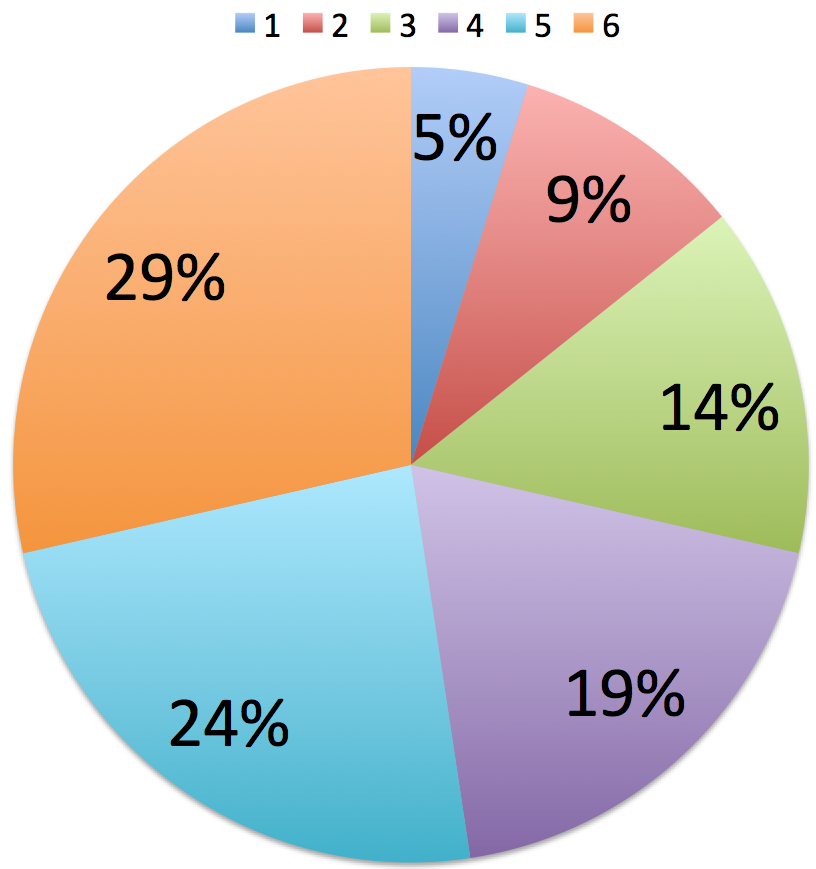
\includegraphics[scale=0.6]{grafiek1.png}\caption{De conversatie opgedeeld in 6 delen, met elk hun procentueel aandeel in de conversatie.}
\label{1}
\end{figure}

We analyseren de conversatie aan de hand van 4 onderdelen. Ten eerste bespreken we het volgens 
de onderdelen van de roos van Leary, vervolgens toetsen we het aan de verschillende niveaus van de 
communicatie. We vervolgen met een blik te werpen op de variabele soorten interventies we kunnen 
toepassen op conversaties. Afsluiten doen we met de inbreng van de begeleider te 
plotten over het tijdsverloop.
\newpage
\subsection{De roos van Leary}
Aan de hand van de roos van Leary kunnen we uitmaken waar de gesprekspartners, 
in dit geval de leerkracht en de bijlesstudent, zich bevinden ten opzichte van 
elkaar. We kunnen afleiden wie boven of onder de andere staat. We kunnen ook aanduiden of ze 
gedrag vertonen om samen of tegen te werken. Op basis van dit 
communicatieparadigma analyseren we onze dialoog.\\

In het eerste deel begint de dialoog zeer gemoedelijk, en vertonen leerkracht en 
bijlesstudent samengedrag. Dit keert echter zeer snel: de leerkracht wil weten 
of de bijlesstudent ooit al examens van wiskunde heeft afgelegd. De leerkracht reageert bij het vragen of hij nog nooit heeft meegedaan,
 onbewust vrij kortaf op het vorige antwoord. Onbewust speelt een verborgen vooroordeel: `Iemand die nog nooit de moeite heeft gedaan om mee te doen aan het examen, wat zou die ooit kunnen slagen?'. 
 Dit blijkt uit de intonatie (en de lichaamstaal). Hierdoor positioneert de leerkracht zich onbewust tegen en nog steeds boven de 
 leerling. De leerling merkt dit en dat manifesteert zich ook in een 
 `tegen'-reactie. De leerkracht beseft echter dat dit een uitschuivertje was, 
 want een `tegen'-reactie is niet bevorderlijk voor een kennismakingsgesprek, 
 dat toch constructief hoort te zijn. Bijgevolg herpakt hij zich meteen vanaf 
 \emph{tought unit} 9. De rest van dit gespreksgedeelte verloopt dan ook terug 
 in een constructieve sfeer. Om de student aan te moedigen om vooral veel te 
 vertellen, situeert de leerkracht zich in \emph{tought unit} 17 op het onder, 
 samen-niveau, wat volgend gedrag aanduidt. Samenvatten hebben we dit eerste deel 
 samengevat in een taartdiagram die het samen- \& tegen-gedrag met elkaar 
 vergelijkt. Je vindt het taartdiagram in Figuur \ref{2}.\\
 \begin{figure}[h]
  \centering
  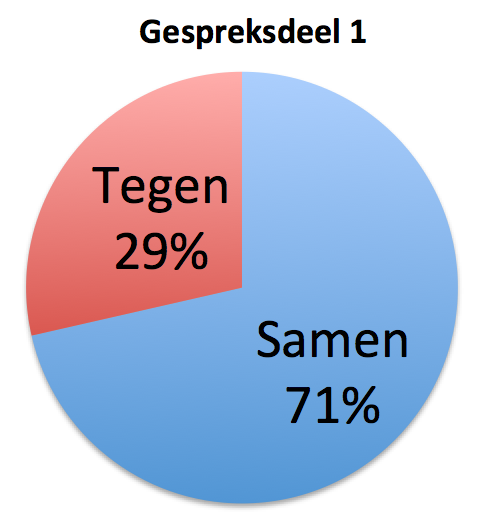
\includegraphics[scale=0.8]{grafiek2.png}\caption{Gespreksdeel 1: analyse van 
het samen- \& tegen-gedrag van de actoren.}\label{2}
\end{figure}

Vermits het tegen-gedrag in het eerste gespreksdeel eigenlijk uitschuiver was, 
herpakt de leerkracht zich en komt er in het hele gesprek in het geheel geen 
tegen-gedrag meer voor. Hieruit kunnen we concluderen dat samen-gedrag daadwerkelijk samen gedrag uitlokt. Dit is duidelijk 
toepasbaar op deze conversatie. Het omgekeerde telt volgens de theorie uiteraard 
ook, maar hiermee kwamen we nauwelijks in aanraking.\\

Laten we nu eens kijken naar het aantal keren dat elke positie op de roos van 
Leary ingenomen worden door zowel de leerkracht als de bijlesstudent. We hebben 
dit voor het eerste gespreksdeel alvast in Figuur \ref{3} in een grafiek gegoten. 
Uit deze grafiek is duidelijk af te leiden dat de leerkracht zich hoofdzakelijk 
in de boven positie bevindt, tenzij om de student aan te moedigen om door te 
vertellen. Dit is logisch omdat de leerkracht ook de leidinggevende is. De student stelt zich steeds onder
de leerkracht of maar meestal samen, wat duidt op een goede medewerking. De \emph{tought units} 
die tegen-gedrag laten blijkben bespraken we reeds in de vorige paragraaf.\\

\begin{figure}
  \centering
  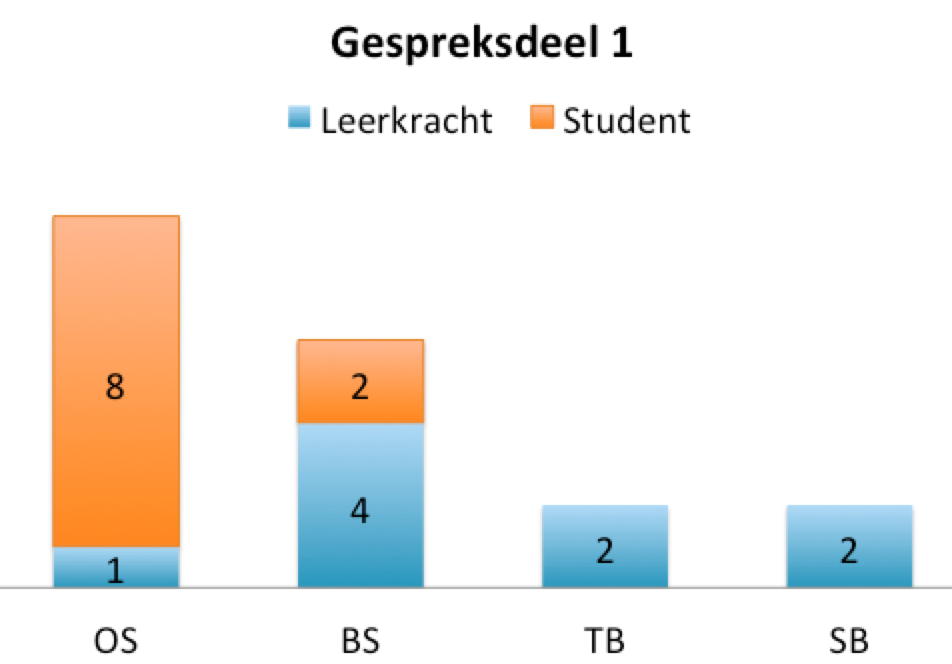
\includegraphics[scale=0.6]{grafiek3.png}\caption{Gespreksdeel 1: analyse van 
de tought units ingedeeld volgens de categorieën van de roos van Leary.}\label{3}
\end{figure}
Tot slot doen we nog eens zo'n analyse van de \emph{tought units} ingedeeld volgens de roos van Leary, maar dan 
voor gespreksdeel 3. Het resultaat hiervan zie je in de grafiek in figuur 
\ref{4}. Concreet hebben we het in het gesprek over de hoe de bijlesstudent zich voelt tijdens de lessen wiskunde, of hij al dan niet meekan en over hoe de lessen georganiseerd zijn (verschil hoor/werkcollege,..). 
Hier is het resultaat helemaal wat je verwacht bij een 
kennismakingsgesprek: beide gesprekspartners vertonen voortdurend samen-gedrag. De positie onder wordt bijna uitsluitend door
de bijlesstudent waargenomen, de leerkracht  staat meestal bovenaan. Enkel als 
de leerkracht een actieve luisterhouding wil aannemen en de student wil 
aanmoedigen om dingen te vertellen, vertoont de leerkracht onder-gedrag. De 
bijlesleerling daarentegen reageert op dit onder-gedrag ook vaak met 
onder-gedrag, zijn positie in het gesprek verandert nauwelijks. Deze analyse van 
deel 3 komt bijna volledig overeen met de analyse voor deel 2, 4, 5 en 5. We 
behandelen deze delen bijgevolg ook niet apart.
\begin{figure}
  \centering
  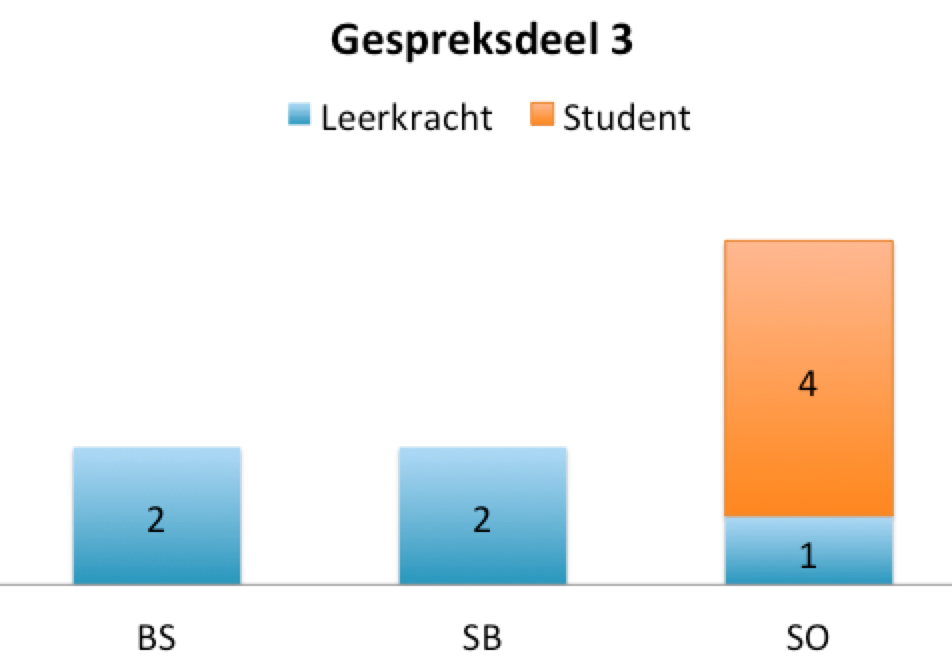
\includegraphics[scale=0.6]{grafiek4.png}\caption{Gespreksdeel 3: analyse van 
de tought units ingedeeld volgens de categorieën van de roos van Leary.}\label{4}
\end{figure}
\newpage
\subsection{Communicatieniveaus}
Bij elke manier van communicatie zijn er vier niveaus van belang. Deze zijn: relatie, inhoud, 
procedure en emotie. Vandaar de benaming RIPE-model. Deze niveaus vormen een 
veerkrachtig evenwicht en ondersteunen het proces. Het is vanzelfsprekend dat wanneer er een 
onderdeel hiervan ontbreekt het de conversatie niet ten goede komt. Men stelt deze vier niveaus voor 
als een vierkant met centraal een cirkel in verwerkt. Deze laatste is uiteraard symbool voor het proces. 
\begin{figure}[h]
  \centering
  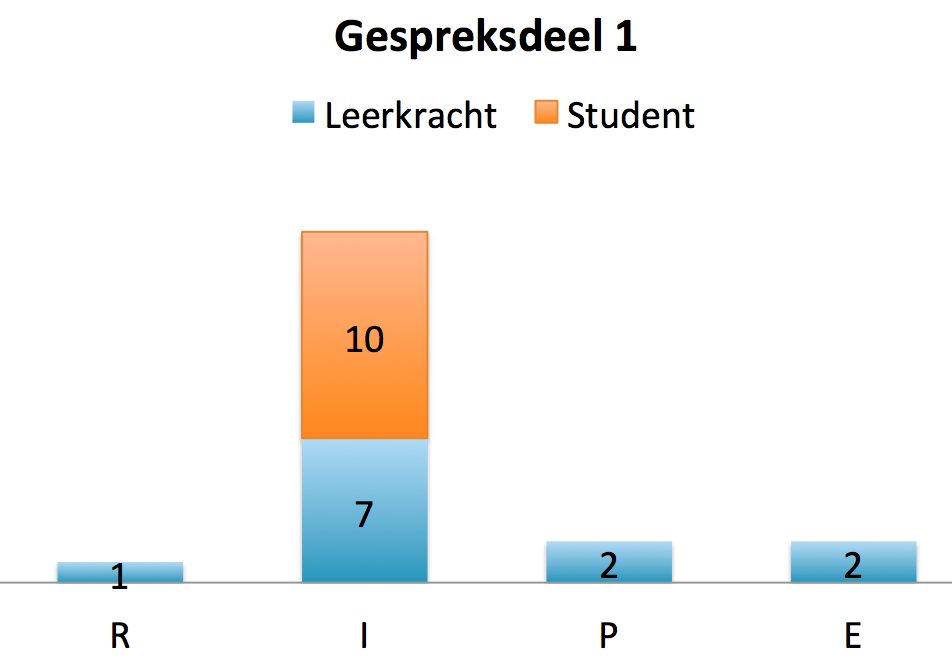
\includegraphics[scale=0.6]{grafiek5.png}\caption{Gespreksdeel 1: analyse van 
de tought units volgens RIPE-model.}\label{5}
\end{figure}
Alweer maakten we een schematisch overzicht van het eerste gespreksdeel in 
Figuur \ref{5}. Het inhoudelijk communicatieniveau neemt de bovenhand. De 
bijlesstudent situeert zichzelf uitsluitend op dit niveau. Het relatieniveau (interactieniveau), is 
buiten een bevestiging van de leerkracht wanneer de student de vakinhoud 
vertelt, totaal afwezig. Het procedureniveau in dit gespreksdeel situeert zich 
bij het verwelkomen en het stellen van de eerste vraag. Het niveau van de emotie bevindt zich bij het ontstaan
van een irritatie bij de leerkracht als de bijlesstudent antwoordt dat hij nog nooit naar een examen is geweest. `Weer eentje
die denkt dat je zonder iets te doen, het zal halen', denkt hij stiekem bij zichzelf. \\

Wat we hier in gespreksdeel 1 kunnen aanschouwen zijn
de typische ingrediënten van een kennismakingsgesprek.  Het relatieniveau is 
uitsluitend aanwezig om de student op zijn gemak te stellen en ontbreekt voor de 
rest totaal: dit is zeer logisch om dat de student en de leerkracht mekaar 
voordien nauwelijks kenden. Het inhoudelijk communicatieniveau neemt een dominante positie, normaal voor een vrij formeel kennismakingsgesprek. In zo'n formele 
setting van een intakegesprek ontbreekt vaak het emotionele niveau, en 
inderdaad: op een kleine uitschuiver in het eerste gespreksdeel na (de leerkracht wou zijn irritatie eigenlijk 
verstoppen), ontbreekt die voor de rest totaal in andere gespreksdelen. \\

Alweer geven we ook een grafiek van gespreksdeel 3 mee in Figuur \ref{6}, omdat deze zeer goed 
overeenkomt met de gespreksdelen 2, 4, 5 en 6 en aldus een goed beeld van het 
gesprek geeft. Concreet hebben we het in het gesprek over de hoe de bijlesstudent zich voelt tijdens de lessen wiskunde, of hij al dan niet meekan en over hoe de lessen georganiseerd zijn (verschil hoor/werkcollege,..). 
We komen tot dezelfde conclusies, al ontbreekt het emotioneel niveau nu totaal. 
Alweer zorgt de leerkracht voor het procedurele aspect, en bevindt de student zich enkel op 
het inhoudelijke niveau. Het relatieniveau wordt alweer door de leerkracht 
waargenomen om de student te stimuleren om vooral verder te vertellen.\\

\begin{figure}
  \centering
  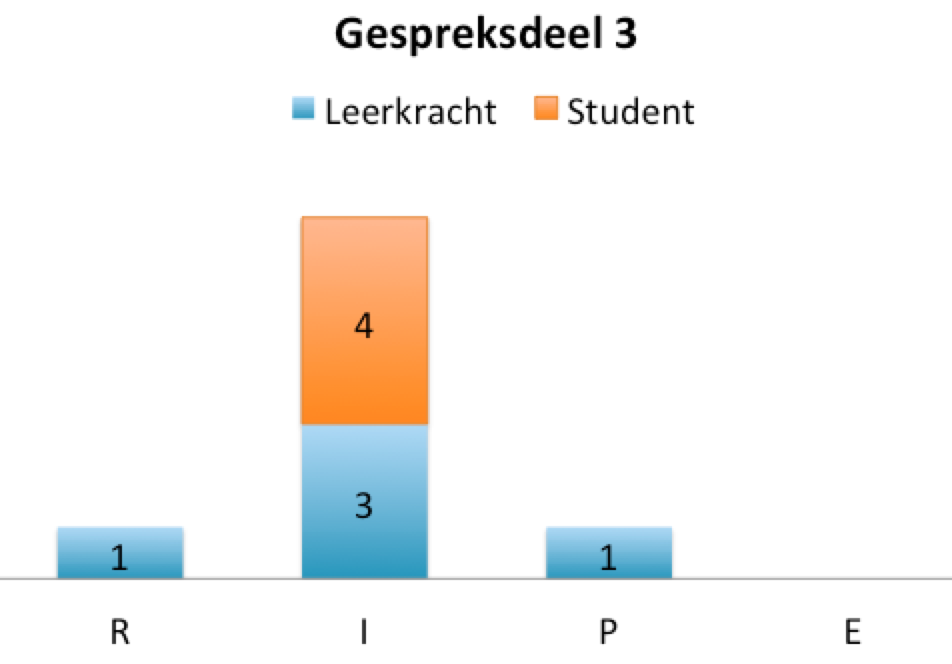
\includegraphics[scale=0.6]{grafiek6.png}\caption{Gespreksdeel 3: analyse van 
de tought units volgens RIPE-model.}\label{6}
\end{figure}

Binnen de niveaus in de communicatie kunnen we nog twee andere onderverdelingen maken. Deze 
van de bovenstroom en de onderstroom. De bovenstroom symboliseert de inhoud van het gesprek 
waar de onderstroom gelijk staat aan het betrekkingsniveau. In dit gesprek wordt de bovenstroom 
voornamelijk gevoed door de bijlesstudent. Terwijl de onderstroom in handen van de leerkracht komt. Als 
we dit samenleggen met het RIPE-model kunnen we quasi stellen dat de bijllesstudent de I-interacties voor 
zijn rekening nam wanneer de leerkracht instond voor de RP(E)-interacties. 
\newpage
\subsection{Interventiecategorieën}
In dit onderdeel van de analyse behandelen we de wijze waarop de begeleider kan interveniëren 
in de conversatie. Gebruikelijk worden er twaalf vaardigheden onderscheiden. De eerste is zich 
openstellen en de laatste die we op het continuüm plaatsen is opleggen. De volgorde van deze categorieën 
werd zorgvuldig bepaald. Van de eerste naar de laatste gebeurt er een verschuiving in de bijdrage van 
een van de partners, dit resulteert in een effect op de gespreksruimte. Hier gaan we later dieper op 
in.\\

We geven in Figuur \ref{7} de verschillende interventiecategorieën gebruikt in gespreksdeel 1 op een 
taartdiagram. Het resultaat is kenmerkend voor een intakegesprek. We zien dat de 
leerkracht meteen aanvangt met enkele vragen die vooral willen informeren. Met 
44\% is informeren dan ook de meest dominante interventie. Wat hier ongewild 
aan bod komt in het eerste gespreksdeel is het oordelen. Het oordelen neemt 9\% maar liefst de tweede plaats in. 
Ongewild is de leraar geënerveerd wanneer de student aangeeft nog nooit aan examen te hebben 
deelgenomen. Deze interventie van de leerkracht past in feite helemaal niet bij 
een kennismakingsgesprek. Door te oordelen daalt de ruimte van de student stevig in het gesprek. De leerkracht eist dan zelf meer ruimte op. Als de leerkacht
vragend aansluit op iets wat de student voorheen vertelde, blijft de inbrengt van de student nog steeds groter dan de inbreng van de leerkracht.
Gelukkig ziet de leerkracht dit ook snel zelf in en 
herpakt hij zich. Dit interventietype komt dan ook niet meer voor in het verdere 
gesprek.\\
\begin{figure}[h]
  \centering
  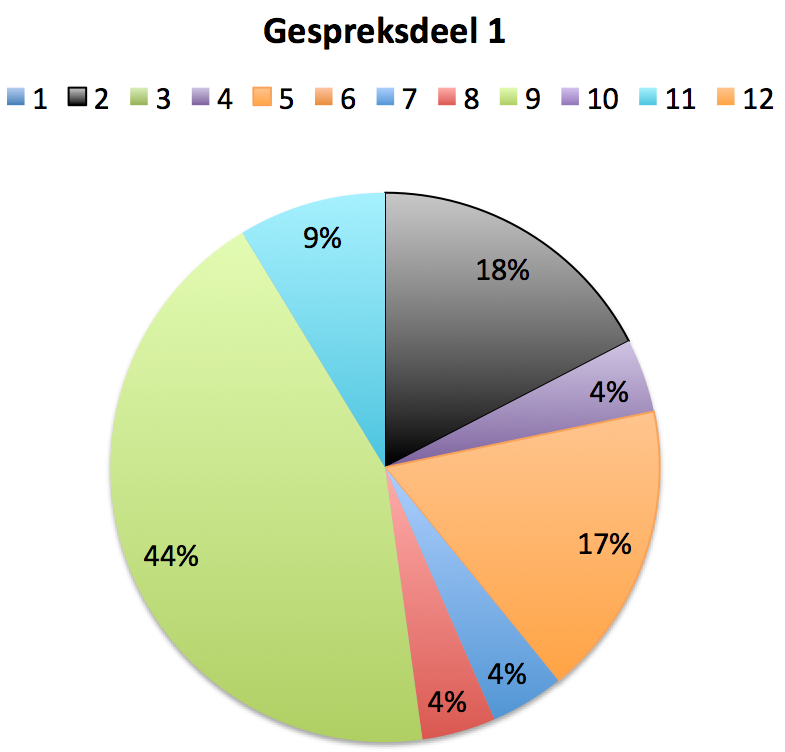
\includegraphics[scale=0.6]{grafiek7.png}\caption{Gespreksdeel 1: taartdiagram met het aandeel van de verschillende interventiecategorieën.}\label{7}
\end{figure}

Kijken we verder, naar gespreksdeel 3 bijvoorbeeld in Figuur \ref{8}, dan zien 
we pas echt dat het gesprek de volledige gedaante van een intakegesprek draagt. Concreet hebben we het nu in het gesprek over 
 hoe de bijlesstudent zich voelt tijdens de lessen wiskunde en hoe ze exact 
 georganiseerd zijn. We zien hier echt een intakegesprek want de typerende 
 interventies informeren en vragend toevoegen scoren hier
 respectievelijk 56\% en 33\%. Dit zijn dus duidelijk de dominante interventies in het gesprek. Merk ook op dat gespreksdeel 3 heel goed lijkt op de andere gespreksdelen, met uitzondering van 1. 
 Ook het actief luisteren krijgt zijn plaats: interventiecategorie 2 scoort 
 11\%. Aan de hand van knikjes en bevestigingen probeert de leerkracht de 
 student uit te nodigen om verder te praten. Ze moedigen hem aan om zijn verhaal 
 te vertellen.
 \begin{figure}[h]
  \centering
  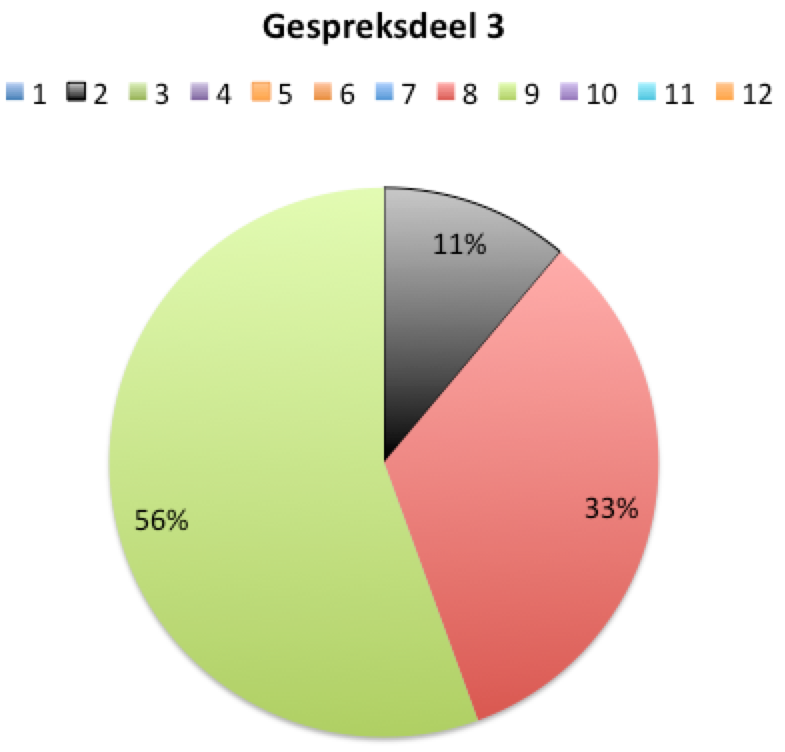
\includegraphics[scale=0.6]{grafiek8.png}\caption{Gespreksdeel 3: taartdiagram met het aandeel van de verschillende interventiecategorieën.}\label{8}
\end{figure}
\newpage
\subsection{Inbreng van de leerkracht versus bijlesstudent}
In Figuur \ref{9} krijg je overzicht van de inbreng van de leerkracht versus die van de bijlesstudent met 
betrekking tot het tijdsverloop. Op de $X$-as staan de \emph{tought units}, op 
de $Y$-as de duur in aantal seconden van de \emph{tought unit}. De leerkracht 
bekleedt de gele lijn, de bijlesstudent de groene.
\begin{figure}[h]
  \centering
  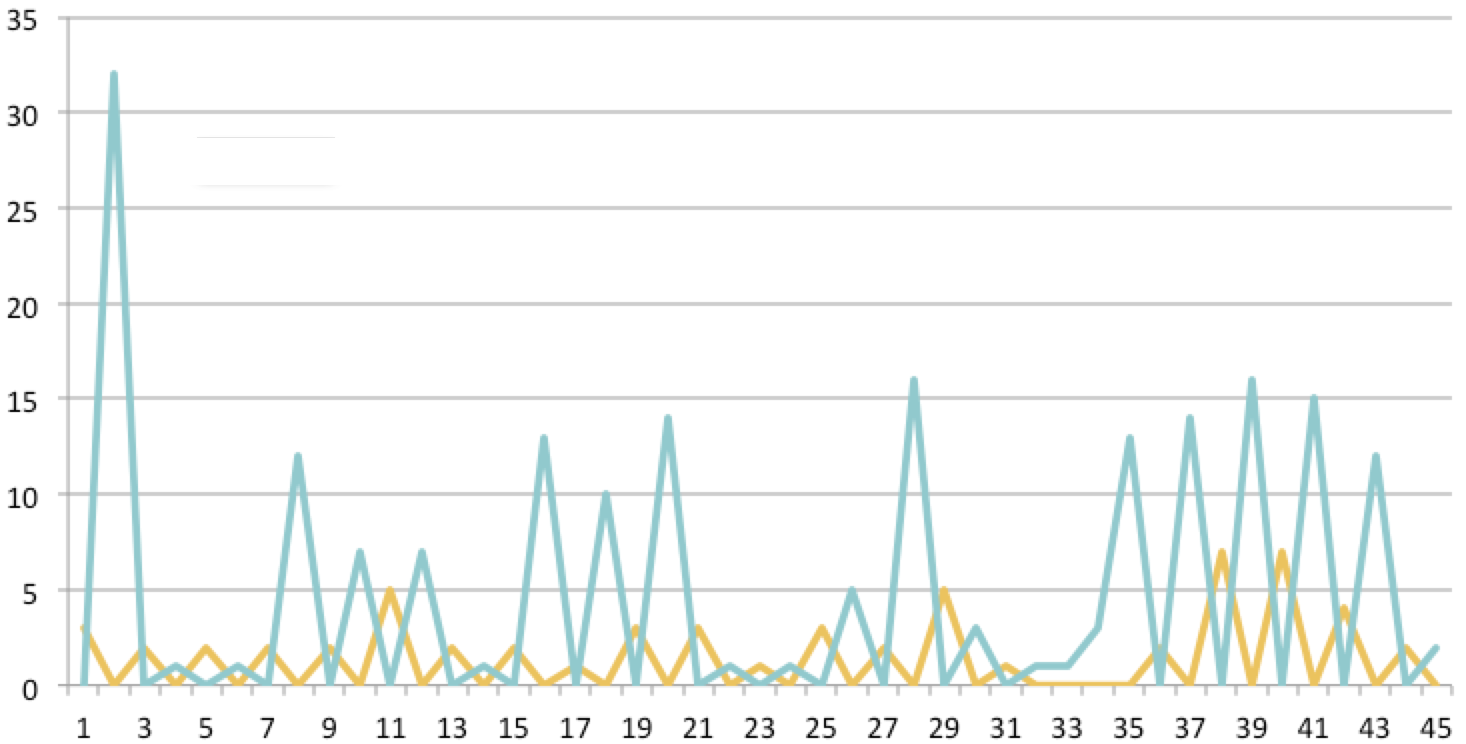
\includegraphics[scale=0.5]{grafiek9.png}\caption{Inbreng van de begeleider versus de bijlesstudent geplot over het tijdverloop. De $X$-as geeft het nummer van tought unit aan, de $Y$-as zijn duur in seconden. Leekracht is de gele lijn, bijlesstudent de groene.}\label{9}
\end{figure}

De algemene inbreng van de leerkracht zweeft tussen het vragend aansluiten en het informatie geven. 
De laagste pieken die we bij hem aantreffen in deze grafiek bevinden zich op de plaats van het luisteren. 
De bijlesstudent piekt in het hele gesprek, met \emph{tought unit} 2 als 
absolute uitschieter, met een duurtijd van 33 seconden. Alweer kenmerkt deze 
grafiek een intakegesprek, de student is veel meer en veel langer aan het woord.
\newpage
\section{Suggesties voor verbetering}\footnote{Ik blijf in deze paragraaf over `de leerkracht' spreken, maar uiteraard bedoel ik hiermee mezelf. Ik tracht 
hiermee een consistente naamgeving van de actoren in het gesprek na te streven.}
Dit gesprek kan gecatalogeerd worden onder een typisch kennismakingsgesprek. De 
leerkracht wil aan de hand van vragen een beeld krijgen over de nieuwe 
bijlesleerling.  Toch is het zeker geen ideaal gesprek. Volgende zaken stonden 
een goed kennismakingsgesprek in de weg:
\begin{itemize}
  \item Zowel de leerkracht als de bijlessleerling kenden elkaar `van zien' 
  reeds vooraf. Het gevolg is dat dit kennismakingsgesprek meteen met de deur in 
  huis valt en meteen over wiskunde gaat, wat het niveau van de procedure schaadt. Er was geen rustig aanloopmoment in
  dit gesprek met wat luchtige vragen als: `Wat zijn je hobby's', `Waar woon je?',... 
  \item Het procedureel niveau is over de hele lijn problematisch. 
  \begin{itemize}
    \item Het gesprek begint erg vreemd en confronterend voor de bijlesleerling door meteen te vragen of de bijlessleerling 
    al ooit een examen heeft meegedaan van wiskunde. Dit is meer een vraag voor 
    op het einde.
    \item Omgekeerd valt het op dat de vraag `Wat verwacht je van mij als 
    bijlesleerkracht' eigenlijk een ideale opener van dit gesprek was geweest, 
    terwijl die vraag pas op het einde gesteld wordt. Het had veel logischer 
    geweest.
    \item De leerkracht spring enorm van de hak op de tak, van de verwachtingen 
   van de bijlesstudent over de leerkracht, wordt er ineens overgeschakeld naar 
   het cursusmateriaal en zo zijn er nog vele voorbeelden te vinden. Het lijkt 
   erop dat de leerkracht wel weet wat hij wil vragen, maar hier nooit structuur 
   in aanbracht. Dit maakt het gesprek chaotisch en oppervlakkiger.
     \item De leerkracht 
  pikt te weinig op de gegeven antwoorden. Het lijkt of er een lijstje van te 
  vragen zaken in zijn hoofd zit en hij dat gewoon afgaat. Dit heeft als 
  voordeel dat de leerkracht de bijlesleerling vrijuit laat praten, maar het 
  staat toch een goede interactie in de weg.

  \end{itemize}  
  \item De plaats van het gesprek was niet ideaal, we zaten al meteen aan het 
  bureel van de bijles. Dit had eigenlijk een gesprek moeten zijn met een 
  drankje erbij om rustig af te tasten.
  \item Het feit dat het gesprek opgenomen werd, was zeker voor de bijlesstudent 
  in het begin een rem op de spontaniteit.
  \item Bij de indeling van het gesprek volgens de roos van Leary was ik me er niet van bewust dat ik vaak in 
de boven samen positie plaatste. Ik had me meer samen boven en dus helpend kunnen opstellen in 
plaats van leidend. Anderzijds was dit eigen het soort van intakegesprek waarin ik mij bevond.
\item Op interventieniveau moet ik opletten met de lichaamstaal en de intonantie die leidt tot een onbewuste 
beoordeling van de bijlesstudent. Toen de student aan het gesprek zei dat hij 
nog nooit had deelgenomen aan een wiskundexamen, had ik al meteen een lage dunk van de 
student. Zoiets mag je niet laten blijken, het zet een rem op de constructieve 
sfeer die eigen moet zijn aan intakegesprek.
\item Op het gebied van het actief luisteren had ik meer stiltes mogen laten vallen in het gesprek en zoals gezegd iets meer mogen inpikken op het gezegde. Ik heb 
nogal snel de neiging om de vaardigheid van het luisteren of terugkoppelen toe te passen. Meer moeite 
heb ik met stiltes. Deze zijn soms echter noodzakelijk binnen een gesprek om iemand bijvoorbeeld de 
kans te laten een ogenblik te reflecteren. Ik dacht uitnodigende reacties te geven maar achteraf gezien 
bleken deze oordelen te zijn. Nu heb ik ingezien welke reacties ik moet geen om het uitnodigende 
effect te bekomen. Het inleven in de gevoelens van mijn gesprekspartner en het achterwege laten van 
mijn eigen ideeën, lijken me goed gelukt. 

\end{itemize}
Samengevat leidt dit tot volgende leerpunten voor mezelf:
\begin{itemize}
  \item Ik moet ook de structuur van het gesprek voorbereiden, niet alleen de 
  inhoud;
  \item Ik moet zorgen voor een geschikte locatie voor een gesprek, hier 
  moet ook op voorhand over nagedacht worden;
  \item Ik moet de leiding van het gesprek soms meer aan de andere overlaten, 
  niet alles te strak in handen willen hebben,
  \item Ik moet gefocust blijven tijdens het gesprek en proberen mijn intonatie en lichaamstaal neutraal te houden, ook al heb ik binnenin een (ver)(be) oordeling van de gesprekspartner. 
  Als deze niet ter zake doet, moet deze niet getoond worden. Dit kan het 
  gesprek belemmeren.
\item Ik moet nog meer actief luisteren en meer inpikken op wat er gezegd wordt.
\end{itemize}
 \end{document}

